\documentclass[12pt, oneside, a4paper]{article}

\usepackage[utf8]{inputenc}
\usepackage[round]{natbib}
\usepackage{amsthm}
\usepackage{amssymb}
\usepackage{float}
\usepackage{tabularx}
\usepackage[toc,page]{appendix}
\usepackage{cleveref}
\usepackage{graphicx}
\usepackage{enumitem}
\usepackage{tikz} % To generate the plot from csv
\usepackage{pgfplots}
\usepackage{tabulary}
\usepackage{multicol}
\usepackage{caption}
%\usepackage[nottoc,notlot,notlof]{tocbibind}

%fonts
\usepackage[T1]{fontenc}
\usepackage{charter}
\usepackage[expert]{mathdesign}

% page formatting
\usepackage{titlesec}
\newcommand{\sectionbreak}{\clearpage}
\renewcommand{\baselinestretch}{1.5} 
\captionsetup{labelsep=newline}

% make captions on top
\usepackage{float}
\floatstyle{plaintop}
\restylefloat{table}


\theoremstyle{definition}
\newtheorem{ftsdef}{Definition}
\newcolumntype{R}{>{\raggedleft\arraybackslash}l}%

\title{Econometric Modelling using \\Fuzzy Time Series Analysis}
\author{Michael Gallagher}

% thank khurshid, brian, sam, probably mick

\begin{document}

\maketitle

\listoffigures

\listoftables

\tableofcontents

\newpage

\section{Introduction}

%``Man is still the most extraordinary computer of all.'' - John F. Kennedy.

This project explores the use of fuzzy logic to perform technical analysis on a financial time series. Technical analysis is financial analysis where past price is used to forecast future price movements. It is a widely used but controversial form of analysis. Econometric theories such as the efficient-market hypothesis claim that the price of a security reflects all currently available information about that security, and making investment decisions based on past data can not achieve greater than average returns. In mitigation, a review of the literature indicates that trading strategies that implement technical analysis can consistently generate profits. However, many of the techniques identified have been in use for more than 50 years. Although algorithmic trading has taken hold in finance, new technical analysis techniques which can be easily understood by analysts have not emerged.

This project evaluates the performance of several fuzzy time series models when used for forecasting financial time series. These models are expressed using linguistic terms which can be understood by an expert. They utilise fuzzy time series analysis in their design, which identifies regular patterns in a time series and uses these to forecast observations. The models which are studied are derived from the literature. Variations to these models are introduced as a result of research on technical analysis in financial markets. Naive time series forecasting models are also evaluated for comparison. The design of each model is found in \cref{design}.

A fuzzy time series framework is developed for designing, modifying and testing the proposed fuzzy time series models. \Cref{implementation} discusses the technical implementation of this framework. \Cref{results} evaluates the performance of the models.

\section{Literature Review}

The digital revolution has changed economics substantially. In the 1960s a huge amount of financial data suddenly became available. Economic theory which needed to be evaluated manually could now be tested and verified thoroughly and systematically, ``liberating econometricians from their mechanical calculators'' \citep{fama}. Yet despite the means to test and verify financial models, there is still disagreement about economic theory among academics and professionals.

One area of disagreement is the accuracy of the efficient markets hypothesis, discussed in \cref{emh}. The efficient market hypothesis proposes that the price of a financial security reflects all information publicly available for that security. As a result it is impossible to make a consistent profit by analysing public information, such as identifying or revenue performance or identifying an upward trend on a chart of price.

Although there is a large body of evidence supporting an efficient markets model, it's validity is an extremely controversial area in economic science. Behavioural Finance analysts point to bubbles and crashes as evidence against market efficiency. They argue that behavioural psychology causes irrational swings in prices away from fundamental values. 

The divide in opinions among this issue can be seen by the results of the 2013 Nobel Prize in Economic Science where two of the winners, Eugene Fama and Robert Shiller, were leading figures in the competing fields of Behavioural Finance and Efficient Markets respectively. Eugene Fama commented in his speech that ``no available evidence resolves this issue in a way that convinces both sides''.

\Cref{ta} discusses Technical Analysis, a form of financial analysis where past price movements are studied and used to forecast future movements. This includes popular analysis methods such as identifying a trend in a graph and trading based on how close price is to technically significant points such as the 52-week low. As discussed in \cref{tahist}, it began as a way of linking movement patterns in price to certain market sentiment. In its current form it is a mix of old practices, statistical reasoning, empirical observations and intuition. Specific techniques are discussed in \cref{app:tatechniques}.

Technical analysis has also seen a lot of debate in the economic world, partly because it goes directly against the efficient markets model. Yet a significant amount of positive research has emerged as well as many theoretical explanations for its use, discussed in \cref{taperformance} and \cref{tahumanz}.

``You don't remember important facts and you don't remember because nobody is talking about it ... we forget and so we repeat mistakes from the past'' claimed Robert Shiller in his Nobel Prize acceptance speech, shortly after Fama. These repeated mistakes are what interest technical analysts. The goal is to identify any regularities in financial markets that can be used to forecast future price. 


The digital revolution has not affected technical analysis as much as might have been expected. Automated technical trading algorithms and artificial intelligence models have been developed and have demonstrated great predictive power. Yet these algorithms create extremely complex trading models which are incomprehensible to a human, so human traders use the classic technical trading tools that are intuitive and suited to our visual pattern recognition abilities.

The models studied in this project are intended to be easier understood by an analyst. The models utilise fuzzy logic and fuzzy set theory in which complex models are reasoned using human linguistic terms. Fuzzy set theory is a branch of set theory used in fuzzy logic where values have a degree of membership in a set, instead of either being in the set or not as in classic set theory. This adds a degree of fuzziness when using these sets, as values are 'kind-of' in a set to different degrees. Human linguistics map very well to these fuzzy sets. People use linguistic terms such as 'tall' or 'heavy' to describe objects. The boundaries for these terms are fuzzy. For example, a man who is $180cm$ tall may be described as 'kind-of' tall as well as 'kind-of' average, and he may be described as more tall than average.

Fuzzy logic captures the meaning of human linguistic terms and can express operations in a way humans can easily understand. It understands when values and sets are similar but different, which allows us to fuzzily compare if items are 'kind-of' the same. These two features make fuzzy logic excellent for performing visual pattern recognition. It can understand the patterns that humans look for as well as allow for small differences between patterns observed.

\Cref{fts} discusses fuzzy time series analysis. In fuzzy time series analysis, observations on a time series are mapped onto fuzzy sets, each set representing a range of values on the time series to different degrees of membership.
Changes from one fuzzy set to another are recorded as a relationship between these fuzzy sets. Once all the desired relationships are identified they are grouped together and can be used to forecast fuzzy values.

Forecasting with a fuzzy time series is done under the premise that changes in the time series that happened previously are likely to happen again. In the basic fuzzy time series model, discussed in \cref{basic}, observations are grouped together and the movements between one observation and the next are recorded as a 'change'. If one observation is fuzzified to fuzzy set $a$, and the next observation is fuzzified to fuzzy set $b$, this is recorded as the fuzzy logical relationship $a \rightarrow b$. Relationships with the same left-hand side fuzzy value are grouped together, and when these values are seen during forecasting, the outcomes of all the relationships in the relationship group are used to forecast values.

Many variations of the basic model have been identified in the literature. \Cref{higher} discusses a higher-order fuzzy time series, where the relationships are computed between observations that are multiple points in time apart. In a $n$-order There are $n$ sets of relationship groups which are used to forecast based on the $n$ most recent observations. A fuzzy intersection is performed on the forecast values, so only fuzzy values that are forecast by all relationship groups are used in the forecasting. This narrows down the values forecast, resulting in a more accurate model of the time series. It also adds another dimension of fuzziness, such that if the past $n$ observations are composed of two or more patterns that have been identified previously, this will be recognised and the outcomes of these patterns will be used for the forecast.

Practical problems for a fuzzy time series have also been examined. \Cref{interval} discusses interval selection in a fuzzy time series. Intervals are divisions in the time series that allow points in the same interval range to be grouped together. The size of intervals is important as too large intervals result in a poor model and too small intervals lose some of the benefit of fuzzy logic.

\subsection{Technical Analysis}
\label{ta}
\begin{figure}[H]
    \centering
    \includegraphics[width=0.8\textwidth]{images/blackwhite.png}
    \caption{Moving-Average Cross Indicator}
\end{figure}

Technical analysis is a form of financial analysis where past price behaviour is used to forecast future price in financial markets. It is one of several methods of analysing financial securities. Other methods include fundamental analysis, which involves analysing the health of a security by viewing information such as company earnings, and sentiment analysis, performing analysis on written text or speech regarding a financial security or market and extracting the sentiment of the author or the market towards it \citep{ahmad2011affective}.

%TODO Technical analysis is studied in this paper for a few reasons...

\cite{foundations} argue that ``the general goal of technical analysis is to identify regularities in the time series of prices by extracting non-linear patterns from noisy data''. Examples of this form of analysis include identifying trends in a graph of price movement, or concluding that a price is unlikely to go lower than the 52-week low. Specific techniques are discussed in \Cref{app:tatechniques}.

\subsubsection{History of Technical Analysis}
\label{tahist}
The use of this form of analysis has been documented for several hundred years. One of the first uses of technical analysis dates back to Japan in the 18th Century. In 1710 Japan's rice market had matured enough to begin using rice coupons instead of trading physical rice. Their receipts were traded constituting the first Futures trades ever recorded \citep[p.~15]{jcct1991}. 

Munehisa Homma was a rice merchant in Japan, who amassed great wealth trading these rice coupons and is sometimes credited as the Father of Japanese Candlestick Charting. Although it is unclear whether Homma actually used Japanese Candlestick Charting techniques, it is recorded that he used the history of price movement to gauge the emotions of the market at the time, ``When all are bearish, there is cause for prices to rise. When everyone is bullish, there is cause for the price to fall''. Following Homma different charting techniques were introduced, until the introduction and popularisation of Japanese Candlestick Charting for technical analysis in the mid 19th Century \citep[p.~18]{jcct1994}.

In the west, Dow Theory was developed and expanded on in the early 20th Century, leading to works such as those by \cite{edwards1948technical} that directly influence technical analysis today.

Even with such a diverse history the use of technical analysis is still a hotly debated topic. Experts and Academics are divided in its use \citep{foundations}, the influential \textit{A Random Walk Down Wall Street} concluding it is as valid as Alchemy when put under scientific scrutiny \cite[p.~159]{randomwalk2012}. Nonetheless, it appears that a significant number of analysts incorporate technical analysis, with a study by \cite{examininguse1997} finding that a mean importance of 35\% was given to technical analysis by respondents in various investment banks and \cite{cheung2000currency} characterising 30\% of Foreign-Exchange traders as Technical Traders. 

\subsubsection{Performance of Technical Analysis}
\label{taperformance}
\cite{taprofitability} performed a comprehensive review of 95 studies of technical trading strategies between 1988 and 2004. While there is a significant number of studies before this, they argue that modern studies ``typically increase the number of trading systems tested, assess risks of trading rules,
perform statistical tests with either conventional statistical tests or more sophisticated bootstrap methods, or both, and conduct parameter optimization and out-of-sample verification''.

\cite{taprofitability} found that of these modern studies, 56 found positive results, 20 obtained negative results and 19 indicated mixed results. 

They offered several theoretical explanations for the positive results. Econometric models such as the noisy rational expectations model postulate that the current price does not reveal all information about a security because of noise, and the market shows a systematic slowness in adjusting to new market information which may be exploited with technical analysis. Behavioural models propose that price is affected by market psychology which can be predicted using technical analysis akin to the original use of technical analysis. Technical analysis charting methods may also be equivalent to non-linear forecasting methods in chaos theory.

They also offered empirical explanations for the results, such as trends in price before news such as central bank interventions, and order flows where the ``take profit'' and ``stop loss'' of orders clusters around round numbers. Other empirical explanations offer the possibility of false positive trading profits. Temporary market inefficiencies may occur, where new trading strategies offer short term gains before they become more widely used and cease to offer an advantage. Also market microstructure deficiencies where studies do not adequately take transaction costs and other market factors into account may lead to inaccurate results. 

\cite{taprofitability} acknowledge that despite the positive evidence and improved procedures, many academics and professional analysts are sceptical about technical analysis and technical trading strategies which utilise it. They point to \cite[p.~25]{assetpricing} who argues that ``trading rules that reliably survive transactions costs and do not implicitly expose the investor to risk have not yet been reliably demonstrated''. Park and Irwin interpret this to mean that the scepticism is due to data snooping problems, where trading strategies over-fit the testing data, and insignificant profits are obtained after making adjustments for transaction costs and risk.

In the professional world, it could be due to the difficulty in experimentally verifying some technical analysis techniques, many of which rely on visual cues in the eyes of an expert. The existence of a pattern is subjective. Experts looking at the same data may see different, sometimes contradictory patterns, fuelling a controversy that technical analysis is nothing more than pseudo-analysis. Also with most studies finding some technical trading strategies successful and many unsuccessful, seemingly without reason, it may be perceived as safer to ignore technical analysis altogether.

\subsubsection{Efficient Market Hypothesis}
\label{emh}
``I believe there is no other proposition in economics which has more solid empirical evidence supporting it than the Efficient Market Hypothesis'' stated \cite{jensen1978some}. The Efficient Market Hypothesis claims that the price of a security is extremely efficient at reflecting most of the information about that security. When news is made public, the market will very efficiently arrive at a price for the security that reflects the impact of the news. This has major consequences; that using technical analysis or fundamental analysis as the basis for an investment portfolio cannot achieve a greater profit than if a random selection of securities were invested in \citep{emhAndCritics}.

While there is a lot of support for this model, strict adherence to it does not offer the complete picture. If the markets were perfectly efficient then the price would simply jump between points as news is made available. In reality there is a large amount of noise, volatility and uncertainty in the market. Very often it is not clear what impact some news should have, how accurate information is and whether the price already reflects the news as it's made available.

\cite{malkiel1970efficient} argue that these issues do not necessarily imply an inefficient market unless there are investors who can consistently make better evaluations of available information. They argue that the hypothesis that the price of a security ``fully reflects'' all available information at any point in time is an extreme null hypothesis, which we do not expect to be literally true. Different efficient market models have been proposed with characteristics that can be evaluated separately, allowing researchers to pinpoint where the hypothesis breaks down. The \textit{weak form} model claims that price reflects all past publicly available information. The \textit{semi-strong form} model claims that the price reflects all past publicly available information and also that price will instantly change as new information is made available. The \textit{strong form} model claims that price reflects all public and non-public information.

The Random Walk Hypothesis proposes that the price of a security represents a 'random walk' around its intrinsic value, and consequently that price movements cannot be predicted. \cite{malkiel1970efficient} describes the random walk model as a ``fair game'' model in which the conditions of market equilibrium can be stated in terms of expected returns, but note that an efficient market does not require a random walk. 

\cite{lo1988} tested the random walk hypothesis by comparing variance estimators of stock market returns. They argue that if prices are generated by a random walk, then the variance of the monthly sample log-price, i.e.\ the variance of the log of the difference in the monthly price must be 4 times as large as the variance of the weekly sample. Their findings strongly reject the random walk hypothesis, but are careful to note that ``this rejection does not necessarily imply the inefficiency of stock-price formulation''.

Almost 30 years ago, \cite{indefenseof} showed that past prices combined with other information, such as non-public information, can achieve unusual profit. They claim that non-price information creates opportunity that can be efficiently exploited using technical analysis. As non-public information is revealed to an investor, it is unclear as to the extent that this information has been revealed. If the investor knows the behaviour that a market would demonstrate had this information was widely distributed, he or she could examine the past price movements and determine a probability that the information has been revealed, and thus determine if there is still opportunity for a profitable investment. While this demonstrates a use for past price data, it only demonstrates use when combined with other valuable information, and thus does not contradict the Efficient Markets Hypothesis that attempting to make profits by exploiting currently available information is futile \citep{taprofitability}.

\subsubsection{Perception}

\label{tahumanz}

Although the evidence supporting technical analysis as a tool for forecasting the market is inconclusive, it is still regarded as an important forecasting tool by many analysts. One of several explanations by \cite[pp.~45-71]{aronson2011evidence} is that humans suffer cognitive biases when determining the significance of visual patterns in their analysis. Many experts believe they can spot visual patterns such as price trends on a graph, and would challenge the claim that these trends are irrelevant.

However when developing or practising a trading system based on patterns, technical analysts can succumb to confirmation bias by giving a higher significance to evidence that supports the pattern they're looking for as opposed to evidence for other patterns that might be available. When determining the efficacy of these systems based on past data, hindsight bias can lead to certain patterns appearing obvious after their formation. This leads an expert to think this pattern is easily detectable, even though while the pattern was forming the evidence for that particular pattern was inconclusive, and possibly pointed to other, contradictory patterns \cite[p.~62]{aronson2011evidence}.

Another explanation is that technical analysis appeals to behavioural psychology. If a large amount of investors are searching for similar patterns, then the subsequent price movement may become a self-fulfilling prophecy. A study by \cite{examininguse1997} finds that 49\% of Foreign-Exchange Technical Analysts surveyed explicitly cite this as a reason. These points are disputed by \cite[p.~162]{randomwalk2012} who states "The problem is that once such a regularity is known to market participants, people will act in a way that prevents it from happening in the future" .

\subsection{Fuzzy Time Series}

\label{fts}

A time series is a set of observations taken sequentially in time. A core characteristic of a time series is that adjacent observations are typically dependent, such that the value of the observation at time $t$ is somewhat dependent on the value at time $t-1$.

A fuzzy time series is a model of a time series that uses fuzzy set theory to find relationships between points on the time series and use these relationships to forecast observations. According to \cite{chen1996forecasting}, "the main difference between a a fuzzy time series and conventional time series is that the values of the former are fuzzy sets and the latter are real numbers".

The typical use of a fuzzy time series is to forecast observations on the time series using historical data. Studies using fuzzy time series have been carried out on forecasting university enrolment \citep{song1993forecasting, song1994forecasting, chen1996forecasting, tsai2000forecasting, chen2004new, cheng2006trend, lee2006pattern, huarng2006ratio, tsaur2012fuzzy}, Stock Market price \citep{huarng2005type, cheng2006trend, lee2006pattern, huarng2006ratio, Chen2007fib, chu2009fuzzy}, Foreign-Exchange rates \citep{tsaur2012fuzzy}, population change \citep{tsai1999study} and temperature \citep{temperatureprediction2000, lee2006pattern}. 

%TODO lo et all candlestick analysis

\subsubsection{Basic Model}
\label{basic}
\cite{song1993forecasting} pioneered the fuzzy time series model providing the definitions for the concept and a method for modelling a time invariant fuzzy time series. The method was shown to be better than the Linear Regression Method for forecasting student enrolments at the University of Alabama. The model fuzzified points on the time series into fuzzy sets and defined fuzzy relations between these sets. They use an arithmetic defuzzification algorithm to interpret the results and claim that ``it is not difficult to jump to the conclusion that in the interpretation of the output results, experience knowledge is still needed''.
 
\cite{chen1996forecasting} improved this model by using simplified mathematical operations instead of computationally expensive max-min composition for defining fuzzy relations. This method, while being more efficient, was also shown to be more accurate than the method proposed by \cite{song1993forecasting}.The steps involved are summarised as follows:

\begin{description}
\item[Step 1] Define a universe of discourse over the maximum and minimum values of observations on the time series and partition it into several intervals.
\item[Step 2] Define fuzzy sets on the universe of discourse. Each fuzzy set consists of each of the intervals to different degrees of membership. Fuzzify the time series into these fuzzy sets.
\item[Step 3] Fuzzify the observations of the time series into the fuzzy set which has a maximum membership for the interval that an observation falls into.
\item[Step 4] Identify movements between adjacent observations on the fuzzy time series as relationships, such the relationship for the sequence fuzzy set $a$ followed by fuzzy set $b$ is recorded as $a \rightarrow b$.
\item[Step 5] Group the relationships based on their left-hand side value. These groups are called fuzzy logical relationship groups.
\item[Step 6] Forecast observations. Let $A_{i}, A_{j}, \ldots, A_{k}$ be fuzzy sets in the fuzzy time series $F(t)(t=1,2,\ldots)$. Let $F(t) = A_{i}$. This step is concerned with forecasting the fuzzy value of $F(t+1)$.
\begin{enumerate}
\item If  $A_i \rightarrow A_k$ is the only fuzzy logical relationship in the fuzzy logical relationship group associated with $A_t$, then $F(t+1)$ is forecast as $A_k$ 
\item If there are multiple fuzzy logical relationships associated with $A_i$ such that $A_i \rightarrow A_{i}, A_{j}, \ldots, A_{k}$, then $F(t+1)$ is forecast as $A_{i}, A_{j}, \ldots, A_{k}$
\item If there are no fuzzy logical relationships associated with $A_i$, then $F(t+1)$ is forecast as $A_i$
\end{enumerate}
\item[Step 6] Defuzzify the forecast fuzzy set using the Centroid method. Practically, this involves calculating the average of the midpoints of each interval which has a maximum membership in each fuzzy set that is forecast for $F(t+1)$
\end{description}

\subsubsection{Higher-Order Models}

\label{higher}

In a first-order time series, described in \Cref{basic}, fuzzy relations are defined between each adjacent point and only the most recent value in a time series is used for forecasting.

An $nth$-order or higher-order fuzzy time series is one where there is a simultaneous relationship between multiple points on the time series, not just adjacent observations. There are fuzzy logical relationship groups defined between all points $1,2,\ldots,n$ spaces in time apart. The most recent $n$ observations are used to forecast fuzzy values, which are then composed and defuzzified.

\cite{tsai1999study} found that a second-order fuzzy time series led to more accurate predictions when forecasting population, particularly when the number of intervals on the fuzzy time series was increased. \cite{tsai2000forecasting} compared the performance of 5 higher-order time series models for predicting university enrolments. They found the higher-order models to be more accurate, with the model increasing in accuracy with every increase in the order of the time series, up to a fifth-order time series.

\subsubsection{Interval Selection}

\label{interval}

Deciding on the size and number of interval partitions on the universe of discourse is an important issue \citep{Huarng2001effective,  huarng2006ratio}. If there are too few intervals, there will be fewer fluctuations in the fuzzy time series \citep{Huarng2001effective} which results in less precise fuzzy logical relationships. Too many intervals can lose some of the benefits of fuzziness with similar patterns not being grouped together.

Many studies use an arbitrarily selected interval size \citep{song1993forecasting, song1994forecasting, chen1996forecasting, tsai2000forecasting, chen2004new}. \cite{tsai2000forecasting} show that when modelling a higher-order fuzzy time series, increasing the number of intervals dramatically improved results. They found that by increasing the number of intervals from $7$ to $19$, the root mean square error of the forecast results fell from $609.22$ to $199.32$. \cite{tsai1999study} found similar improvements when increasing the number of intervals, for both first-order and higher-order fuzzy time series. \cite{chen2004new} proposed a method for forecasting university enrolments which used 13 intervals instead of the usual 7, and an extra step which further divided each interval into 4 parts in order to detect a trend of movement. Although this cannot be attributed solely to increasing the number of intervals, it also demonstrated significantly improved forecasting accuracy. 	

\cite{Huarng2001effective} examined a distribution-based and average-based approach for selecting interval length. Both of these approaches derive the interval length using the absolute difference of any two consecutive observations and ensure that at least half of these differences in the time series are reflected by the intervals. 

Both methods utilise a mapping table to approximate the interval size to the nearest 10. This is called the \textit{base} and is derived from the average first difference. The distribution-based approach plots the distribution of the first differences according to multiples of this \textit{base}. The largest multiple of the base that is smaller than at least half the first-differences is chosen as the interval. The average-based approach involves calculating half of the average first difference, rounding this value to the \textit{base} and using this as the interval.

\cite{Huarng2001effective} found that these approaches resulted in improved accuracy compared to the arbitrarily selected intervals used in prior studies, with the average-based approach performing better than the distribution-based approach. He compared the results of both approaches with 9 arbitrarily chosen but small interval lengths, and found that the average-based approach resulted in the best and second best predictions for university enrolments and the Taiwan Stock Exchange Weighted Index (TAIEX) respectively. They also found that smaller interval lengths did not always result in a more accurate prediction.

\cite{huarng2006ratio} explored an approach to define intervals using the ratios between the absolute differences. The rationale behind using ratios was that the momentum of the time series oscillates more or less depending on the context. The same source of data, such as a stock price, may have different optimal interval lengths depending on the amount of activity of the time series at that time. Using interval lengths that reflect the relative difference between observations takes this into account without using a secondary data source such as volume.

The ratio-based approach was evaluated using the same methodology as used by \cite{Huarng2001effective}. It resulted in the best accuracy for the methods tested when forecasting university enrolment, TAIEX price and inventory stock. It was also found that the optimal interval length changed between data sets from the same data source, and that the ratio-based approach was effective at approximating the optimal length.

\section{Design}

\label{design}

\subsection{Basic Fuzzy Time Series Model}
\label{fts-design}
This section provides the definitions for a basic fuzzy time series model and provides the steps involved for building the model. This model is used as a base from which other models are defined. It is derived from the literature discussed in \cref{basic}, and uses the ratio-based interval selection algorithm to define interval lengths, shown in \cref{ratio}.

\begin{ftsdef}
\label{def1}
Let $Y(t)(t= \ldots,0,1,2, \ldots)$, a subset of $\mathbb{R}$, be the universe of discourse on which fuzzy sets $f_i(t)(i=1,2,\ldots)$ are defined and let $F(t)$ be the set of $f_i(t)(i=1,2,\ldots)$. Then $F(t)$ is a fuzzy time series on $Y(t)(t= \ldots,0,1,2, \ldots)$.
\end{ftsdef}

\begin{ftsdef}
\label{def2}
Suppose $F(t)$ is caused by $F(t-1)$, then this relation can be expressed as $F(t)=F(t-1) \circ R(t,t-1)$, where $R(t,t-1)$ is the fuzzy logical relationship between $F(t-1)$ and $F(t)$, denoted as $F(t-1) \rightarrow F(t)$.
\end{ftsdef}

\begin{ftsdef}
\label{def3}
All fuzzy logical relationships in a fuzzy time series can be grouped into fuzzy logical relationship groups based on their left-hand side value. These groups are denoted as $F(k) \rightarrow F(m), F(n), \ldots, F(l)$
\end{ftsdef}

In \cref{def1}, $Y(t)$ represents a time series. The range of the observations in this time series is called the universe of discourse. $f_i(t)$ are fuzzy sets over the universe of discourse, consisting of the all the intervals defined on the universe and the membership of each interval in that fuzzy set. $F(t)$ is the collection of all of these fuzzy sets. This collection of fuzzy sets at any point $t$ on a time series is called a fuzzy time series.

\begin{figure}[H]
	\centering
	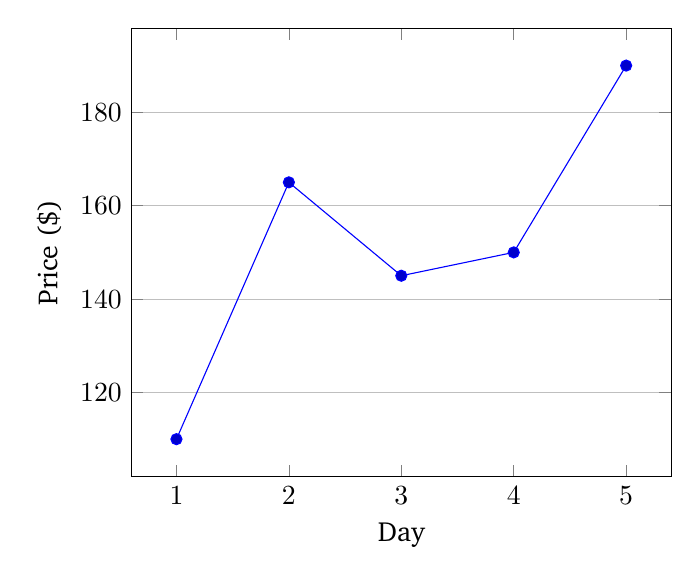
\begin{tikzpicture} 
		\begin{axis}[xlabel=Day,ylabel=Price (\$), ymajorgrids, trim axis left, trim axis right] 
			\addplot coordinates { 
				(1,110) 
				(2,165) 
				(3,145) 
				(4,150) 
				(5,190) 
			}; 
		\end{axis} 
	\end{tikzpicture}
	\caption{5-day closing stock price Y(t)}
	\label{graph}
\end{figure}

Consider the daily closing stock price for a company $Y(t)(t=1,2,\ldots,5)$, such that $Y(1) = 110$, $Y(2) = 165$, $Y(3) = 145$, $Y(4) = 150$ and $Y(5) = 190$. A graph of the time series is shown in \cref{graph}.

The universe of discourse needs to cover the range between the highest and lowest values that are being considered, which in this case is $110$ and $190$. To simplify the explanation of the example, $[100 \ldots 200]$ is used as the universe of discourse.

This example considers one linguistic variable which indicates the performance of a stock. The universe of discourse is partitioned into equal length intervals, $\left\{u_1, u_2,\ldots,u_k\right\}$, shown in \cref{int}.
%TODO could really do with explanaing ``membership''
\begin{table}[H]
	\center
	\begin{tabulary}{1.0\textwidth}{ LCL }
	\hline
	$u_1$ & $=$ & $[100 \ldots 120]$ \\
	$u_2$ & $=$ & $[120 \ldots 140]$ \\
	$u_3$ & $=$ & $[140 \ldots 160]$ \\
	$u_4$ & $=$ & $[160 \ldots 180]$ \\
	$u_5$ & $=$ & $[180 \ldots 200]$ \\
	\hline
	\end{tabulary}
	\caption{Intervals}
	\label{int}
\end{table}

Fuzzy sets are then defined which are the values of the linguistic variable ``Performance", $very\_low$, $low$, $mid$, $high$ and $very\_high$. These fuzzy sets consist each interval and its grade of membership in the fuzzy set, shown in \cref{fuzzy_sets}.

\begin{table}[H]
	\center
	\begin{tabulary}{1.0\textwidth}{ LCL }
	\hline
	$very\_low$ & $=$  & $1/u_1 + 0.5/u_2 + 0/u_3 + 0/u_4 + 0/u_5$ \\
	$low$ & $=$ & $0.5/u_1 + 1/u_2 + 0.5/u_3 + 0/u_4 + 0/u_5$ \\ 
	$med$ & $=$ & $0/u_1 + 0.5/u_2 + 1/u_3 + 0.5/u_4 + 0/u_5$ \\
	$high$ & $=$ & $0/u_1 + 0/u_2 + 0.5/u_3 + 1/u_4 + 0.5/u_5$ \\
	$very\_high$ & $=$ & $0/u_1 + 0/u_2 + 0/u_3 + 0.5/u_4 + 1/u_5$ \\
	\hline
	\end{tabulary}
	\caption{Fuzzy Sets}
	\label{fuzzy_sets}
\end{table}

From \Cref{def1} we say that $F(t)$, derived from $Y(t)$, is a fuzzy time series of the linguistic variable ``Performance'' with fuzzy sets $f_i(t) (i=1,2,\ldots)$ as its values. \Cref{def2} states that, for a first order fuzzy time series, there is a relationship $R$ between $F(t-1)$ and $F(t)$ for any time $t$ in the time series. This is called a fuzzy logical relationship and is denoted as $F(t-1) \rightarrow F(t)$.

Following from the example, $Y(t)$ is mapped to the fuzzy time series $F(t)$. Each observation in the time series is mapped a fuzzy set based on the interval that the observation falls into having a maximum membership in that fuzzy set. Using the fuzzy sets defined in \cref{fuzzy_sets}, the fuzzy mappings for the time series are $F(1)=low$, $F(2)=high$, $F(3)=med$, $F(4)=med$ and $F(5)=very\_high$. The fuzzy logical relationships can be shown as follows: 

\begin{table}[h]
	\center
	\begin{tabular}{ l l l }
	\hline
  	$low \rightarrow high$  \\
  	$high \rightarrow med$ \\
  	$med \rightarrow med$ \\
  	$med \rightarrow very\_high$ \\
  	\hline
	\end{tabular}
	\caption{Fuzzy Logical Relationships}
\end{table}

\Cref{def3} states that fuzzy logical relationships which share the same left-hand side value may be grouped into fuzzy logical relationships groups. The fuzzy logical relationship groups for the example are as follows:

\begin{table}[h]
	\center
	\begin{tabular}{ c c c c }
	\hline
  	Group 1: & $low$ & $\rightarrow$ & $high$ \\
  	Group 2: & $med$ & $\rightarrow$ & $med, very\_high$ \\
  	Group 3: & $high$ & $\rightarrow$ & $med$ \\
  	\hline
	\end{tabular}
	\caption{Fuzzy Logical Relationship Groups}
\end{table}

These relationships are used to forecast observations in time. Taking $t+1$ as the point in time to be forecast, we forecast a fuzzy value for $F(t+1)$ using the fuzzy logic relationship grouping where the left-hand side is $F(t)$. If there is no matching fuzzy logical relationship group for $F(t)$, then $F(t)$ is forecast.

The forecast value or values for $F(t+1)$ are defuzzified by taking the mean of the midpoints of the intervals which have a maximum membership in the forecast fuzzy sets. This crisp value is forecast for $Y(t+1)$.

To illustrate, if $F(t)$ is $med$, then the fuzzy logical relationships group with a matching left-hand side is Group 2. From this the forecast fuzzy values for $F(t+1)$ are $med$ and $very\_high$. The intervals with a maximum membership in these fuzzy sets are $u_3$ and $u_5$ respectively. The midpoint of these intervals are $150$ for $u_3$ and $190$ for $u_5$, with a mean value $\frac{150 + 190}{2}=170$. This crisp value is used as the forecast.

\subsection{Higher-order Fuzzy Time Series Model}
\label{higher-order}

This section defines a higher-order fuzzy time series and a formal method forecasting using this model. A higher-order fuzzy time series, discussed in \cref{higher}, is an extension of the basic model. It is a more precise as a separate list of values are forecast for each of the most recent $n$ observations in an $n$-order fuzzy time series, and only values common to all forecasts are used. It also adds another element of fuzziness to the analysis as patterns only need to be partially completed to be identified.

\begin{ftsdef}
\label{def5}
Let $F(t)(t=1,2,\ldots)$ be a fuzzy time series. Suppose $F(t)$ is caused by $F(t-1),F(t-2),\ldots,F(t-n)$ simultaneously, then $F(t)$ is a higher order, $n$-order, fuzzy time series and the fuzzy logical relationships are denoted as $F(t-n), \ldots, F(t-2), F(t-1) \rightarrow F(t)$.
\end{ftsdef}

\Cref{def5} defines a higher-order fuzzy time series. \cite{tsai1999study} developed a procedure which captures the essence of a higher-order fuzzy time series while maintaining the simplicity of first-order calculations.

In an $n$-order fuzzy time series, $F(t)$ is caused by $F(t-1)$, $F(t-2)$, $\ldots$, and $F(t-m)$ simultaneously. The $n$ fuzzy logical relationships for $F(t)$ are obtained in the same manner as a first-order model. The relationships can be represented as follows:

\begin{table}[H]
	\center
	\begin{tabular}{ c }
	\hline
  	$F(t-1) \rightarrow F(t)$ \\
  	$F(t-2) \rightarrow F(t)$ \\
  	\vdots \\
  	$F(t-n) \rightarrow F(t)$ \\
  	\hline
	\end{tabular}
	\caption{Higher-Order Fuzzy Logical Relationships}
\end{table}

The relational function for a fuzzy logical relationship $F(t-k) \rightarrow F(t)$ is expressed as $R^{n}_{k}(t)$. In an $n$-order fuzzy time series, for any forecast $F(t)$, there are $n$ relational functions $R^{n}_{\ \ 1}, R^{n}_{\ \ 2}, \ldots, R^{n}_{\ \ n}$ where $R^{n}_{\ \ k}=R(t,t-k)$. Note that in $R^{n}_{\ \ k}$, the $n$ indicates what order model the relation is for. The $k$ represents the fuzzy relation between $F(t-k)$ and $F(k)$, for all $k={1,2,\ldots,n}$. 

For example, the relational matrix representing the fuzzy logical relationships between observations 2 points in time apart on a third-order fuzzy time series could be shown as in \cref{2-order-rels}.

\begin{table}[H]
	\center
	\begin{tabular}{ c }
	\hline
  	$R^{3}_{\ \ 2}(1) = F(1) \times F(3)$ \\
  	$R^{3}_{\ \ 2}(2) = F(2) \times F(4)$ \\
  	\vdots \\
  	$R^{3}_{\ \ 2}(k) = F(k) \times F(k-2)$ \\
  	\hline
	\end{tabular}
	\caption{2-Order Fuzzy Logical Relationships}
	\label{2-order-rels}
\end{table}

\Cref{2-order-rels} shows the equations for the 2-order fuzzy logical relationships. For a 3-order fuzzy time series, the fuzzy logical relationships for $R^{3}_{\ \ 1}(t)$ and $R^{3}_{\ \ 3}(t)$ will also need to be computed for all times $t$. Once these values are obtained, $R^{n}_{\ \ m}(m=1,2,\ldots)$ represents the set of $n$ fuzzy time series models which were calculated by analysing observations at different points in time apart. Each of these contains a set of $m$ fuzzy logical relationship groups which are used simultaneously for forecasting. 

\begin{table}[H]
	\center
	\begin{tabular}{ c }
	\hline
  	$F_{i1} = F_{i-1} \circ R^{n}_{\ \ 1}$ \\
  	$F_{i2} = F_{i-2} \circ R^{n}_{\ \ 2}$ \\
  	\vdots \\
  	$F_{in} = F_{i-n} \circ R^{n}_{\ \ n}$ \\
  	\hline
	\end{tabular}
	\caption{Forecast Values}
	\label{forecasting}
\end{table}

\Cref{forecasting} shows the collection of fuzzy values forecast by the fuzzy logical relationship group $R^{m}_{\ \ k}$ at time $i$ for all $k=1,2,\ldots,n$. Since the above relations happen simultaneously, the forecast for $F(i)$ is the fuzzy intersection of all $F_{ik}$, which are the forecast fuzzy values common to each order of fuzzy logical relationship groups used. These values are then defuzzified as in \Cref{fts-design}.

\subsection{Moving-window Model}

This section describes... It is designed... (section in progress)

A $n$-length moving window fuzzy time series is one in which the $n$ most recent observations in a time series are treated as one observation. It differs from a higher-order fuzzy time series in that it crisply identifies patterns as being a particular sequence and records the relationship between the entire pattern and the outcome as the fuzzy logical relationship.

For illustration, a the fuzzy logical relationships for a $2$-order fuzzy time series and a $2$-length moving-window fuzzy time series will be compared.

Consider the following fuzzy time series sample $F(t)(t=1,2,\ldots,5)$:

\begin{table}[H]
	\center
	\begin{tabular}{ c }
	\hline
  	$F(1) = a$ \\
  	$F(2) = b$ \\
  	$F(3) = b$ \\
  	$F(4) = c$ \\
  	$F(5) = a$ \\
  	\hline
	\end{tabular}
	\caption{Fuzzy Time Series Sample}
\end{table}

where $a$, $b$ and $c$ are fuzzy sets.

In a 2-order time series, there are 2 sets of fuzzy logical relationship groups identified, the relationships between observations 1 and 2 points in time apart:

\begin{multicols}{2}
\begin{table}[H]
	\center
	\begin{tabular}{ c c c c }
	\hline
  	Group 1: & $a$ &  $\rightarrow$ & $b$ \\
  	Group 2: & $b$ & $\rightarrow$ & $b, c$ \\
  	Group 3: & $c$ &  $\rightarrow$ & $a$ \\
  	\hline
	\end{tabular}
	\caption{1-order FLRGs}
\end{table}
\columnbreak
\begin{table}[H]
	\center
	\begin{tabular}{ c c c c }
	\hline
  	Group 1: & $a$ & $\rightarrow$ & $c$ \\
  	Group 2: & $b$ & $\rightarrow$ & $c, a$ \\
  	\hline
	\end{tabular}
	\caption{2-order FLRGs}
\end{table}
\end{multicols}

In comparison, the fuzzy logical relationship groups For a 2-length moving window fuzzy time series are as follows:

\begin{table}[H]
	\center
	\begin{tabular}{ c c c c }
	\hline
  	Group 1: & $a, b$ & $\rightarrow$ & $b$ \\
  	Group 2: & $b, b$ & $\rightarrow$ & $c$ \\
  	Group 3: & $b, c$ & $\rightarrow$ & $a$ \\
  	\hline
	\end{tabular}
	\caption{2-length moving window FLRGs}
\end{table}

The 2 most recent observations are taken and matched to the appropriate relationship group which is used to forecasts values. This is different to the 2-order fuzzy time series which would use the fuzzy intersection of the values forecast by each set of fuzzy logical relationships as the forecast.

A $n$-length moving window fuzzy time series can also be a $n$-order fuzzy time series. The results from this variation are studied.

\subsection{Change-analysis Model}

This section describes... It is designed... (section in progress)

One of the goals of the project is to identify technical patterns in an econometric time series. Technical patterns are sequences of movements in a time series, typically forming a visual pattern, which are used to forecast price change. 

The proposed fuzzy time series model will recognise technical patterns which consist of the same values, i.e.\ that form technical pattern at the same point along the $y$-axis of a time series. This is useful as it accounts for ``significant'' price levels as discussed in \Cref{app:tatechniques}. 

However this does not identify technical patterns consisting of movements of price, which is what many visual patterns are. Identifying changes between observations results in patterns which can be applied to any point on the time series, e.g.\ the pattern $up,up,up,down,up$.

The change-analysis model uses other time series models to perform analysis. This model is differentiated by virtue that it analyses the changes of the time series instead of the time series itself. By generating a new time series composed of the changes of the original time series, the same steps can be used to identify the relationships between changes and forecast changes instead of a crisp price.

To illustrate, \cref{changes} shows a time-series of the changes of \cref{graph}.

\begin{figure}[H]
	\centering
	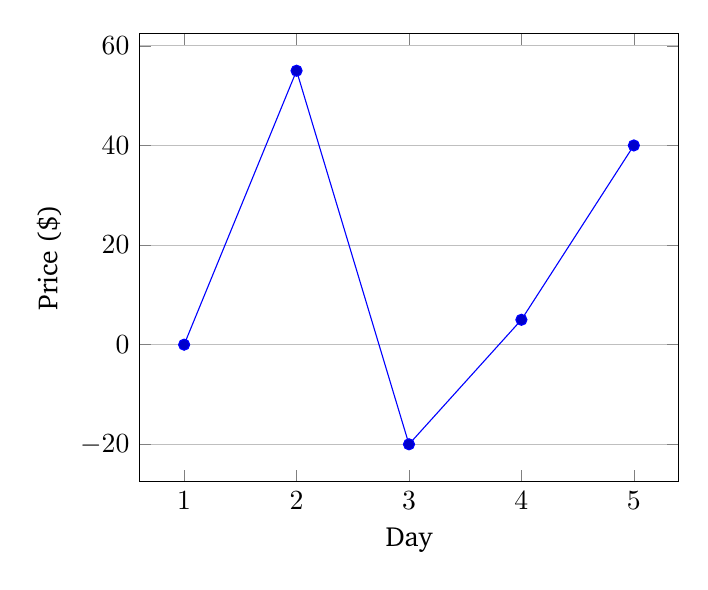
\begin{tikzpicture} 
		\begin{axis}[xlabel=Day,ylabel=Price (\$), ymajorgrids, trim axis left, trim axis right] 
			\addplot coordinates { 
				(1,0) 
				(2,55) 
				(3,-20) 
				(4,5) 
				(5,40) 
			}; 
		\end{axis} 
	\end{tikzpicture}
	\caption{5-day change of price Y(t)}
	\label{changes}
\end{figure}

%TODO talk about the drawbacks of ratio based approach with change analysis

\subsection{Naive models}
\subsubsection{Buy \& Hold}
\subsubsection{Random Walk}

\subsection{Ratio-based Interval Selection}
\label{ratio}

The following method for ratio-based interval selection was studied by \cite{huarng2006ratio}.

\begin{table}[H]
	\center
	\begin{tabularx}{0.5\textwidth}{ X R }
	\hline
  	MIN$(r_1,\ldots,r_{n-1})$ & Base\\
  	\hline 
  	\noalign{\smallskip}
	$\leq 0.05\%$ & $0.01\%$ \\
	$\leq 0.5\%$ & $0.1\%$ \\
	$\leq 5.0\%$ & $1\%$ \\
	\ldots & \ldots \\
	\hline
	\end{tabularx}
	\caption{Base Mapping Table for Ratios}
\end{table}

\begin{description}
\item[Step 1] Calculate the relative difference between adjacent observations such that $r_t=|x_t-x_{t-1}|/x_{t-1}$ for all $t$
\item[Step 2] Determine the $base$ by mapping MIN$(r_1,\ldots,r_{n-1})$ to the base mapping table
\item[Step 3] Plot the distribution for all $r_t$ according to the determined $base$
\item[Step 4] Choose a sample percentile of the relative differences $\alpha$, such as $\alpha=50\%$. Select a $ratio$ which is the smallest relative difference that is larger than $\alpha$
\item[Step 5] Calculate the intervals 

\begin{table}[H]
	\center
	\begin{tabular}{ c }
		\hline
	  	$u_1 = [lower_1, upper_1]$ \\
	  	$u_2 = [lower_2, upper_2]$ \\
	  	\vdots \\
	  	\hline
	\end{tabular}
\end{table}

The beginning of the first interval, $lower_1$, is set to MIN$(x_t)-c$ where MIN$(x_t)$ is the lowest observation and c is some small constant. The $interval\_length$ for the time series is calculated as $interval\_length=(lower_1 \times ratio) - lower_1$. The upper bound of the first interval, $upper_1$, is set to $lower_1 + interval\_length$. The remaining intervals are calculated using the formula $[lower_k,upper_k]=[lower_{k-1}+interval\_length+c, upper_{k-1}+interval\_length+c]$ for all $k=(2,3,\ldots)$.
\end{description}

\subsection{Root Mean Squared Error}

\label{rmse}

The metric used to measure the forecasting accuracy of time series models is a contentious issue. There is often not a consensus around which metric is appropriate \citep{hyndman2006another}.

This paper measures the accuracy of the proposed model with the Root Mean Squared Error (RMSE) as a performance indicator. The RMSE represents the sample standard deviation of the forecasting error and gives an indication of the variance of the forecasting model. RMSE is the most common performance indicator used in the literature allowing the performance of the proposed models to be compared to previous studies. However, it does not support comparing the performance of a model when using different datasets due to RMSE being scale dependent. The formula is given in \cref{rmse}.

\begin{figure}[H]
    \centering
    \caption{RMSE Formula}
    $\sqrt{\frac{\sum_{n}^{t=1}|actual(t)-forecast(t)|^{2}}{n}}$
    \label{rmse}
\end{figure}
 
%make random walk model heterosedastic, as in stock markets do not follow random walks


\section{Implementation}

\label{implementation}

\subsection{Initial Implementation}

The code for the project was built in two separate iterations. The initial implementation was written in MetaQuotes Language 5 (MQL5), a C-like domain specific language for the electronic trading platform MetaTrader 5 (MT5). This language was chosen for the following reasons:

\begin{enumerate}[label=\roman*]
\item The trading platform enables the testing of automated trading strategies using past price data
\item The platform includes an interface for drawing overlays onto charts enabling easier visualisation of trading strategy
\item There is an active community of developers using MQL5 and the earlier MQL4
\item The platform offers the ability to use genetic programming for parameter optimisation across a cluster of remote servers 
\end{enumerate}

The initial implementation was concerned with identifying moving window patterns, i.e.\ a particular series of price changes, and the outcome after these patterns. The design was inspired by initial research into technical analysis and fuzzy time series analysis but did not follow the literature as closely as the models outline in \cref{design}. It was aimed at analysing foreign exchange currency pairs, where typically very small changes would occur between points on the time series. An outline of the method is as follows.

Initially a new time series was generated consisting of the changes between observations. The universe of discourse over this new time series was then divided into intervals. The intervals were derived from the standard deviation $\sigma$ of the time series to give meaning to otherwise arbitrarily selected interval lengths. When evaluating foreign exchange currency pairs the interval length $\frac{\sigma}{25}$ was found to result in the appropriate amount of fuzzy logical relationships groups to adequately model the data.

A fuzzy time series was generated where each observation was the interval which contained a point on the time series of changes. Each sequence of $n$ observations on the fuzzy time series is recorded as an $n$ length moving window, where $n$ is a user defined parameter, and the subsequent observation on the time series recorded as the outcome. Multiple instances of patterns in the time series were grouped together and denoted as $pattern \rightarrow \lbrack outcome\rbrack$ where $\lbrack outcome\rbrack$ represents the list of outcomes discovered after instances of $pattern$.

The intention of this design was to identify moving-window patterns in which the mean of the identified outcomes deviated a statistically significant amount from 0. These patterns would be used as trading rules for an algorithmic trading program. This design was moved away from in favour of a fuzzy logic based approach which appeared to be much more flexible at adapting to different time series.

The code for the implementation was written in a performance-orientated manner. It uses pointer arithmetic wherever possible to avoid memory bottlenecks. This includes ``moving window'' objects sharing memory addresses to fuzzified points on the time series, and functions defined to work with pointers instead of objects. A custom statistical class was also defined due to limitations of MQL5's standard library.

The implementation allowed for MQL5 to be evaluated for the purpose of designing a fuzzy time series. It was found to have several shortcomings:

\begin{enumerate}[label=\roman*]
\label{mql5}
\item Data selection typically limited to foreign exchange and precious metals
\item Data in proprietary format and difficult to verify
\item Very limited standard library and testing frameworks
\item Limited debugging capabilities
\item Large overheads when initiating testing on past data
\end{enumerate}

In particular, it was very difficult to compare the implementation to previous studies due to the platform not supporting testing against arbitrary datasets. The limited standard library also required a significant amount of code to be hand written which would otherwise be provided by the programming language developers. Finally there was a large overhead when running the implementation due to the proprietary testing data being retrieved from a remote server each time the program was run.

\subsection{Final Implementation}

The final implementation of the fuzzy time series framework was written in the python programming language, which was chosen for the following reasons:

\begin{enumerate}[label=\roman*]
\label{python}
\item Dynamically typed object-orientated design allows for a clean, compartmentalised codebase
\item Support for lazy evaluation enables speed optimisations in code which makes heavy use of list manipulation
\item Excellent debugger support for easier development and verification
\item Large standard library including statistical packages
\item Popular in financial institutions
\end{enumerate}

The final implementation incorporates the design specified in \cref{design}. The project involves creating a framework for developing and evaluating different fuzzy time series models. The implementation compartmentalises the different steps involved in designing a fuzzy time series. A general interface describing ``ticks'' on the time series allows the model to take ``builder'' functions and generate a time series that can be interpreted by the application. It can also be instructed to analyse the changes between points on the time series instead of the time series itself. This design allows the rest of the application to function while remaining naive to the original format of the dataset.

Intervals are derived from the generated time series using the algorithms defined in \cref{interval}. The interval calculation code consists of a series of utility methods which perform individual steps for the interval calculation, allowing the algorithm to be modified easily.

The framework supports several variations of the basic fuzzy time series model. It allows for easy development of a higher-order fuzzy time series by treating all fuzzy time series as a higher-order model. It also supports identifying moving-window patterns on the time series and forecasting using these. These models can be converted into higher-order moving-window models. Different composition methods such as fuzzy intersection and fuzzy union can be used when forecasting the results of the higher-order models.

The framework features a testing and results suite. It allows for many different variations to the model to be evaluated simultaneously, including changes to the order of the time series and changes to moving-window length. The simultaneous evaluation is made possible by utilising lazy evaluation in the forecasting code. The results suite evaluates the desired models and outputs information about the forecasting after every tick, including the current RMSE, current mean percentage error, previous observation in the time series, current observation in the time series and the forecast value. These results are outputted to a spreadsheet so the performance of each model over time can be graphed and examined.

The testing suite can perform comparisons with any model that implements a forecasting interface. Two naive models are included in the project, a ``buy \& hold'' model and a ``random walk'' model. The ``random walk'' model analyses the training data and calculates the standard deviation of changes, and uses this standard deviation to generate a Gaussian distribution which is randomly sampled to obtain a forecast value. The ``buy \& hold'' model uses the observation at time $t$ as the forecast for observation time $t+1$.

The code was designed with an object-orientated design. The classes of objects, their methods and general interfaces are shown in \cref{uml}. 

The code was written following style guidelines outlined by \cite{bobmartin}. The project followed good programming practices from this book including regular refactoring of code, methods that ``do one thing'', short purposeful classes, meaningful method and class names and designing code such that comments are made redundant.

\begin{figure}[H]
    \centering
    \includegraphics[width=1.0\textwidth]{images/class_diag_a4_priv.png}
    \caption{UML Class Diagram}
    \label{uml}
\end{figure}
\newpage


\subsection{Fuzzy Logic Toolkit}

A minimal fuzzy logic toolkit was written and implemented for the project. While open source fuzzy logic toolkits exist for python, the fuzzy time series model uses only a small subset of operations that exist in fuzzy set theory and writing a bespoke solution offered several advantages for speed and flexibility.

The toolkit supports fuzzification of observations into fuzzy sets as outlined in \cref{fuzzy_sets}. It supports the fuzzification of both single observations and moving-windows, and understands how to treat moving-windows like single observations in a fuzzy time series.

It provides models for fuzzy sets, fuzzy logical relationships and fuzzy logical relationship groups. It features a ``Manager'' class to create, modify, lookup and organise fuzzy logical relationship groups.

In a higher-order fuzzy time series, there are different managers for each of the orders. These manage their own set of fuzzy logical relationship groups and each forecast a list of fuzzy values independently. The fuzzy logic toolkit supports performing a fuzzy intersection on these sets as outlined in \cref{higher-order}.

Defuzzification involves taking the mean of the intervals that have a membership in the forecast fuzzy sets. The final implementation allows for defuzzifying using intervals that have a membership in the forecast fuzzy sets above a user defined threshold $\alpha$. The performance of the models when $\alpha = 1.0$ and $\alpha = 0.5$ is studied.
% TODO don't forget to actually study them!

\subsection{Optimisation}

\label{optimisations}

\subsubsection{Fuzzy Logic Toolkit Optimisations}

Many speed optimisations were achieved with a fuzzy toolkit that was designed knowing the constraints with which it would be used. Fuzzification, identifying matching fuzzy logical relationship groups and performing a fuzzy intersection required a large amount of $O(n)$ operations. 

Fuzzification of an observation was implemented by iterating through the calculated intervals and identifying which interval had a range that included the observation. This would also be done for each value on a moving-window series. This resulted in $O(n)$ list access times, which in a large time series added a significant overhead. This method was optimised by recognising that by starting at the lowest bound of first interval and counting how many times the $interval\_length$ was added before it was larger than the observation, this count corresponded to the index of the appropriate interval for the observation. This optimised operation resulted in $O(1)$ access times.

It was recognised that most of the operations which involved fuzzy sets only used the interval which had a maximum membership in that fuzzy set. Early implementations iterated through the intervals and queried their membership in the fuzzy set until the maximum member was found. This was a wasteful $O(n)$ operation as most of the intervals have a $0$ membership in a fuzzy set, and only one interval would ever have a maximum membership. In order to optimise this a reference to the interval with a maximum membership in a fuzzy set was stored as a public attribute in the fuzzy set object.

One of the most expensive operations of early implementations was adding and finding the fuzzy logical relationship group for a fuzzy logical relationship during training and forecasting respectively. This operation identified the appropriate fuzzy logical relationship group for the left-hand side of a fuzzy logical relationship and recorded the right-hand side as an outcome of that relationship. Initially this involved iterating through the list of fuzzy logical relationship groups and matching until the correct group was found, or creating a new group if one was not found. This $O(n)$ was very costly with more precise fuzzy time series models due to the abundance of fuzzy logical relationships. 

The code was optimised by creating a hash map using the left-hand side values of the fuzzy logical relationships as the ``key'' in the hash map and the a right-hand side as the ``value''. This was done by creating a hash method for the left-hand side object and using this as a key for a dictionary in python. Checking if an appropriate fuzzy logical relationship group exists could be done by querying the ``keys'' method of the dictionary and the appropriate fuzzy logical relationship group could be accessed directly in $O(1)$ time.

\subsubsection{Lazy-evaluation}

Lazy evaluation is a method of evaluation in programming where an expression isn't evaluated until it's value is required. In python this is achieved with generator expressions and the ``itertools'' python module. Generator expressions generate values in a list as it is iterated over. Methods can yield a ``generator iterator'' to a list instead of the list itself. These generators only generate objects when needed, and support the lazy form of operations such as ``zip'', ``map'' and ``slice'' with the itertools module in python.

This project primarily implements lazy evaluation as it does not require a list be fully computed before it can be acted on, e.g.\ only the first value in a list would be calculated to obtain the head of a list. The results framework takes advantage of this by forecasting many variations to the fuzzy time series model simultaneously. Higher-order and moving-window time series can take from several seconds up to several minutes to run against the whole testing data. With lazy evaluation the current RMSE of each model at some point, e.g.\ after 100 observations, can be obtained. This greatly speeds the process of finding the optimal combination of parameters of a fuzzy time series model for different datasets.

\section{Results \& Evaluation}

\label{results}

% The application of neural networks to forecast fuzzy time series has a time breakdown of comparisons!c

\subsection{Comparison Models}

\section{Conclusion}

\section{Future work}

\appendix


\section{Technical Analysis Techniques}

\label{app:tatechniques}

There are many trading strategies that use technical analysis. Almost any strategy that uses past price movement or behaviour as an indicator for future price counts as a technical trading strategy. Discussed here are 3 techniques that are seen to be widely used in technical trading strategies.

\subsection{Trend Identification}
Moving averages are graph lines that indicate the average price over a fixed period. Different functions can also be used such as calculating a weighted moving average. Its purpose is to smooth the noise in a graph and to identify a trend. A moving average cross is where 2 moving averages are used on a graph, generally with one having a short period indicating current trend and one having a long period indicating overall trend. When the line of the short period crosses the line of the long period it is an indication of a change in trend \citep{brock1992}. Moving averages have been used in many studies on technical trading strategies, with generally positive performance. \cite{taprofitability} found moving average rules showed consistently profitable results in the foreign exchange and futures market, and the most reliable performance in the stock market out of the methods tested.

\subsection{Pattern Identification}
Technical Patterns are visual patterns that appear in a graph of price movement. A Head-and-Shoulders pattern is one where the price represents a persons head and shoulders, where the price shows an approximately symmetrical sequence of five local extrema which correspond to 2 shoulders, 2 necks and a head. The outcome of this pattern is that the price moves down. \cite{foundations} examined 10 of these patterns and found overwhelming significance for the indicators when applied to the Nasdaq stock index. \cite{chang1999methodical} also find a Head-and-Shoulders pattern was profitable, but was outperformed by simpler trading rules such as a moving average indicator. Japanese Candlestick charting is considered to be identifying technical patterns.

\subsection{Price Levels}

\begin{figure}[H]
    \centering
    \includegraphics[width=0.8\textwidth]{images/uptrend.png}
    \caption{Visual Support Line}
\end{figure}

Pivot points, Support and Resistance price levels which are very commonly calculated in industry but have not received significant academic attention \citep[p.~55]{osler2000support}. According to \cite{murphy1999technical}, a support level is ``a level or area on the chart under the market where buying interest is sufficiently strong to overcome selling pressure. As a result, a decline is halted and prices turn back up again''. Resistance is the opposite of support. Often they are levels where the price has had difficulty breaking before, either as static price points (such as the weekly low price) or points where the price meets a trend line that it appears to be bounding off. \cite{brock1992} found strong support for this style of trading strategy.

% \clearpage

\addcontentsline{toc}{section}{References}
\bibliographystyle{apa}
\bibliography{dissertation}

\end{document}
